\documentclass[12pt,a4paper, italian]{article}
\usepackage[italian]{babel}
\usepackage[a4paper, margin=1.97cm]{geometry}
\usepackage{caption}
\usepackage{subcaption}
\usepackage{graphicx}
\usepackage{float}
\usepackage{amsmath}
\usepackage{amssymb}
\usepackage{amsfonts}
\usepackage{physics}
\usepackage{placeins}
\usepackage[hidelinks,linktoc=all]{hyperref}
\usepackage[italian]{cleveref}

\graphicspath{{./images/}}

\title{Relazione di laboratorio di fisica computazionale:\\ il modello di Ising in 2-D}
\author{Giacomo Cicala}
\date{\today}

\begin{document}
\maketitle


\section{Introduzione}
In questo elaborato si analizza il comportamento di un reticolo di spin nel caso di campo magnetico assente, descritto dal modello di Ising:
\begin{equation}
    E = -J \sum_{\langle i,j \rangle} s_i s_j
\end{equation}
dove $s_i = \pm 1$ e gli spin sono disposti su un reticolo bidimensionale quadrato di dimensioni $L \times L = 30 \times 30$.
Il sistema viene studiato nell'ensemble canonico a diverse temperature mediante simulazioni Monte Carlo, sfruttando l'algoritmo di Metropolis con dinamica spin-flip e condizioni al contorno periodiche (PBC). Le grandezze macroscopiche d'interesse monitorate durante l'evoluzione all'equilibrio comprendono:

\begin{itemize}
    \item \textbf{Magnetizzazione media per spin:}
          \begin{equation}
              \frac{\langle M \rangle}{N} = \frac{1}{N} \left\langle \sum_{i=1}^{N} s_i \right\rangle
          \end{equation}

    \item \textbf{Magnetizzazione assoluta media per spin:}
          \begin{equation}
              \frac{\langle |M| \rangle}{N} = \frac{1}{N} \left\langle \left| \sum_{i=1}^{N} s_i \right| \right\rangle
          \end{equation}

    \item \textbf{Energia interna media per spin:}
          \begin{equation}
              \frac{\langle E \rangle}{N} = -\frac{J}{N} \left\langle \sum_{\langle i,j \rangle} s_i s_j \right\rangle
          \end{equation}

    \item \textbf{Calore specifico per spin:} definito a partire dalle fluttuazioni dell'energia:
          \begin{equation}
              c = \frac{\langle E^2 \rangle - \langle E \rangle^2}{k_B T^2 N}
          \end{equation}

    \item \textbf{Suscettività magnetica per spin:} definita a partire dalle fluttuazioni della magnetizzazione:
          \begin{equation}
              \tilde{\chi} = \frac{\langle M^2 \rangle - \langle |M| \rangle^2}{k_B T N}
          \end{equation}
\end{itemize}

\section{Obiettivi}
Lo scopo della simulazione si riassume in cinque punti principali:

\begin{enumerate}
    \item \textbf{Energia e magnetizzazione (singolo flip):} Studiare l'andamento dell'energia media per spin $\langle E \rangle / N$ e della magnetizzazione media $\langle M \rangle / N$ (e del suo valore assoluto) in funzione della temperatura $T$, variandola da $1$ a $4$ con passo $\Delta T = 0.05$ (in unità interne $J=k_B=1$). In questo punto i valori delle medie sono calcolati adottando come step Monte Carlo il singolo tentativo di spin-flip ($N_{\text{tot}}= 900.000$ step totali).

    \item \textbf{Suscettività magnetica:} Calcolo della suscettività magnetica per spin $\tilde{\chi}$ nello stesso intervallo di temperature, sfruttando la relazione con le fluttuazioni della magnetizzazione.

    \item \textbf{Calore specifico:} Determinazione del calore specifico per spin $c$ attraverso due metodi indipendenti: a partire dalle fluttuazioni termiche dell'energia interna e mediante la derivata numerica $\pdv{\ev{E}}{T}$.

    \item \textbf{Energia e magnetizzazione (sweep completo):} Ripetizione del calcolo di $\langle E \rangle / N$ e $\langle M \rangle / N$ ridefinendo lo step Monte Carlo come un intero sweep sequenziale su tutto il reticolo, per un totale di $1000$ sweep.

    \item \textbf{Funzione di autocorrelazione:} Calcolo della funzione di autocorrelazione dell'energia $C_c(t)$ fissando la temperatura a $T = 2$, confrontando l'andamento temporale ottenuto con la dinamica a singolo flip rispetto a quella a sweep completi.
\end{enumerate}

\section{Risultati}
\subsection{Energia e magnetizzazione (singolo flip)}
Per una data temperatura, i valori delle quantità di interesse $A$ sono stati calcolati come medie temporali (per la termalizzazione del sistema sono stati scartati i primi $N_{\text{therm}}=90.000$ step Monte Carlo, ovvero $N_{\text{mis}} = N_{\text{tot}} - N_{\text{therm}}$) mediate a loro volta su $N_{\text{seed}}=10$ seed diversi, ovvero
\begin{equation}
    \langle A\rangle = \frac{1}{N_{\text{seed}}} \sum_{s=1}^{N_{\text{seed}}} \left( \frac{1}{N_{\text{mis}} } \sum_{t =0}^{N_{\text{mis} - 1}} A^{(s)}(t) \right)
\end{equation}
di conseguenza le incertezze dei punti sono state calcolate come
\begin{equation}
    \sigma_{\langle A \rangle} = \sqrt{\frac{1}{N_{\text{seed}}(N_{\text{seed}} - 1)} \sum_{s=1}^{N_{\text{seed}}} \left( \bar{A}_s - \langle A \rangle \right)^2}
\end{equation}
dove $\bar{A}_s$ è il valore medio per il seed $s$.

Si è scelto di rappresentare il grafico della magnetizzazione media in valore assoluto, in quanto su run sufficientemente lunghe è possibile che per sistemi di taglia finita avvengano degli spin-flip globali al di sotto della temperatura critica, portando ad un annullamento del valore medio. I risultati sono riassunti in \cref{fig:e_m_1flip}.
\begin{figure}[H]
    \centering
    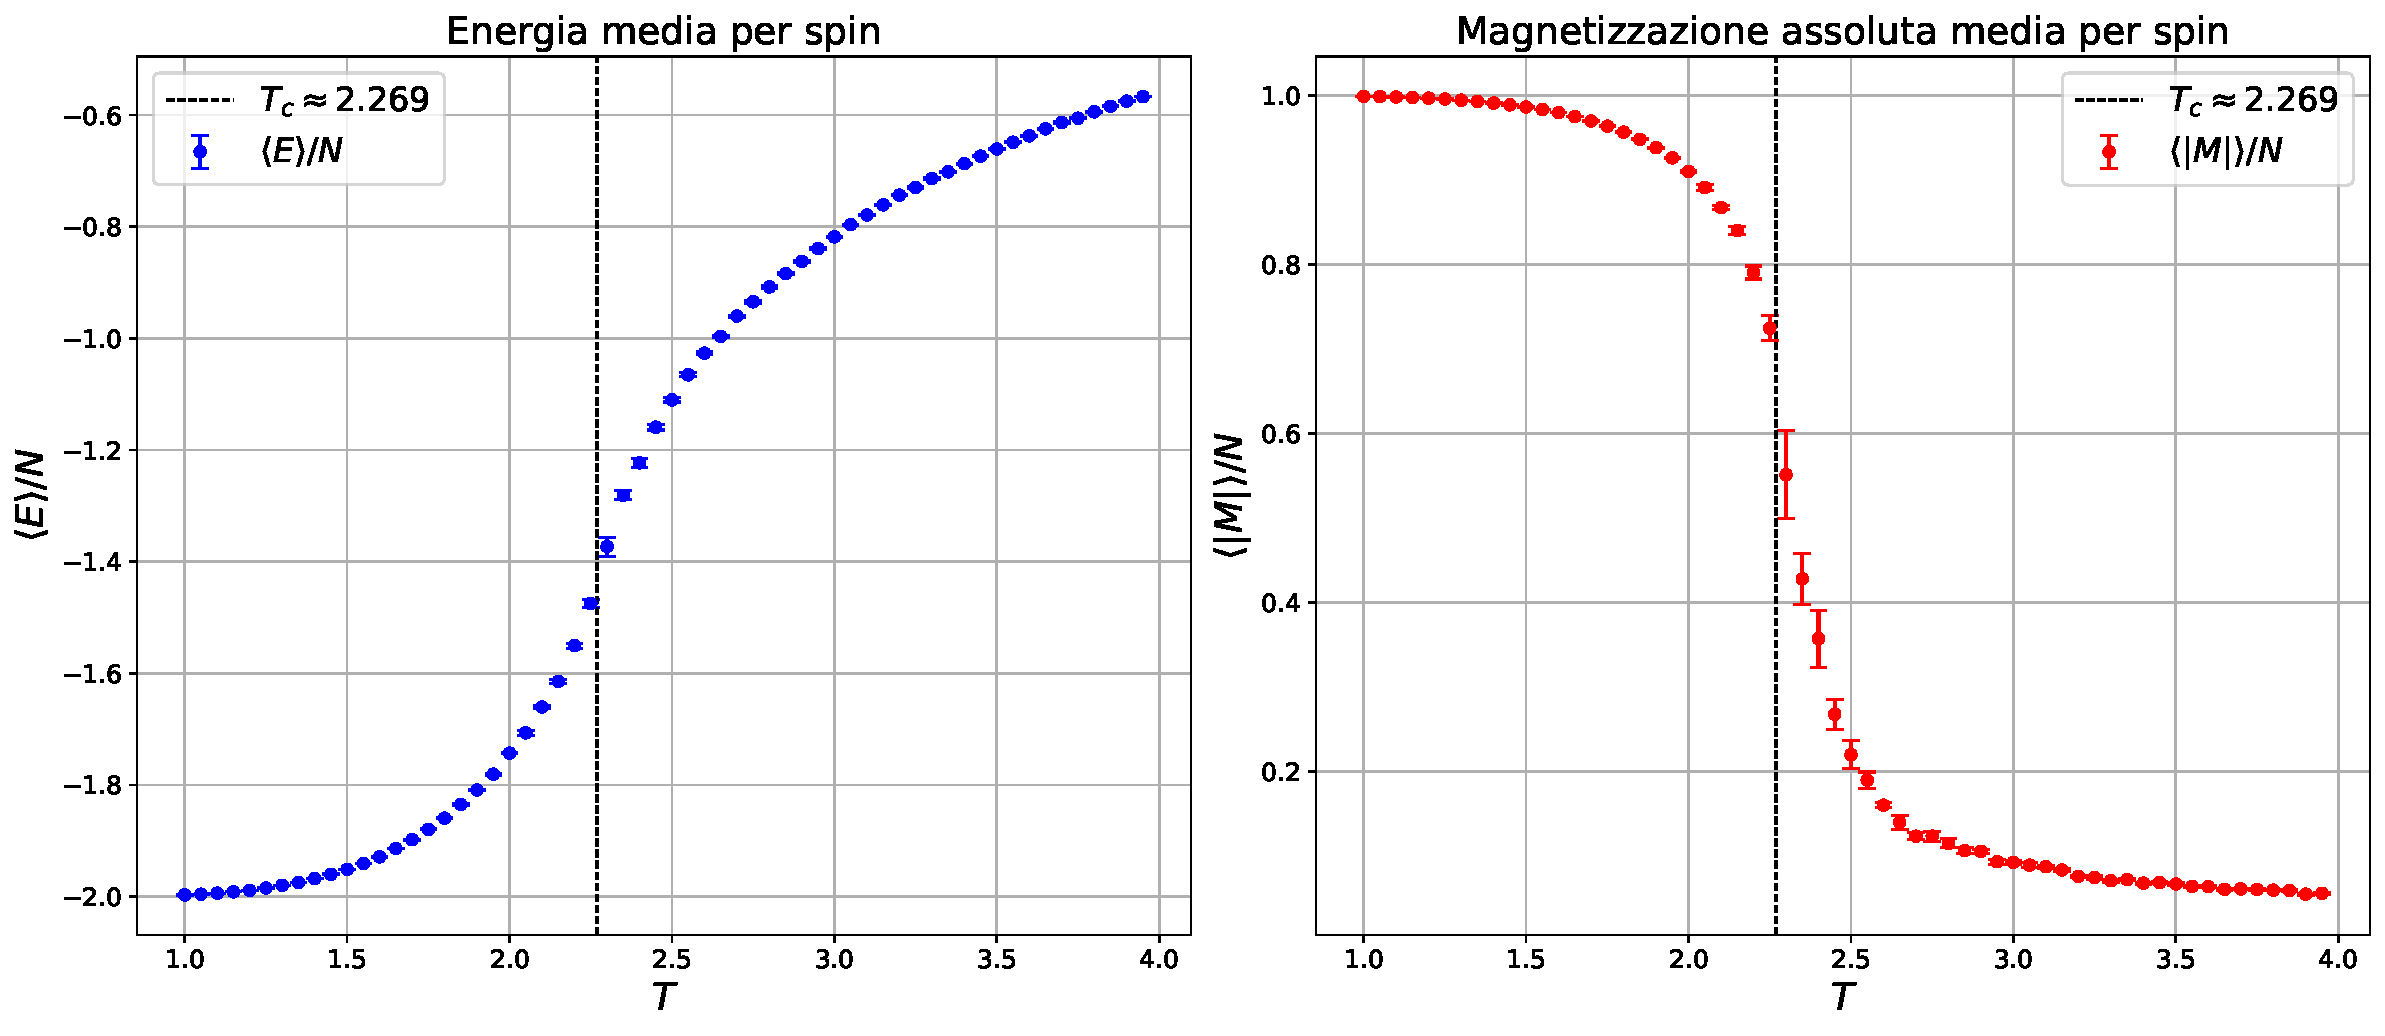
\includegraphics[width=\textwidth]{punto1_energia_magnetizzazione.pdf}
    \caption{Energia media per spin (sinistra) e magnetizzazione assoluta media per spin (destra) in funzione della temperatura in unità interne $J=k_B=1$, nel caso in cui uno step Monte Carlo corrisponda ad un tentativo di spin-flip, mediate su $N_{\text{seed}} = 10$ simulazioni indipendenti.}
    \label{fig:e_m_1flip}
\end{figure}
\FloatBarrier


\subsection{Suscettività magnetica}
Come anticipato precedentemente, il valore della suscettività magnetica è significativo solo quando consideriamo il valore medio della magnetizzazione assoluta.
I parametri della simulazione sono i medesimi del punto precedente; il risultato è riportato in \cref{fig:chi}.
\begin{figure}[H]
    \centering
    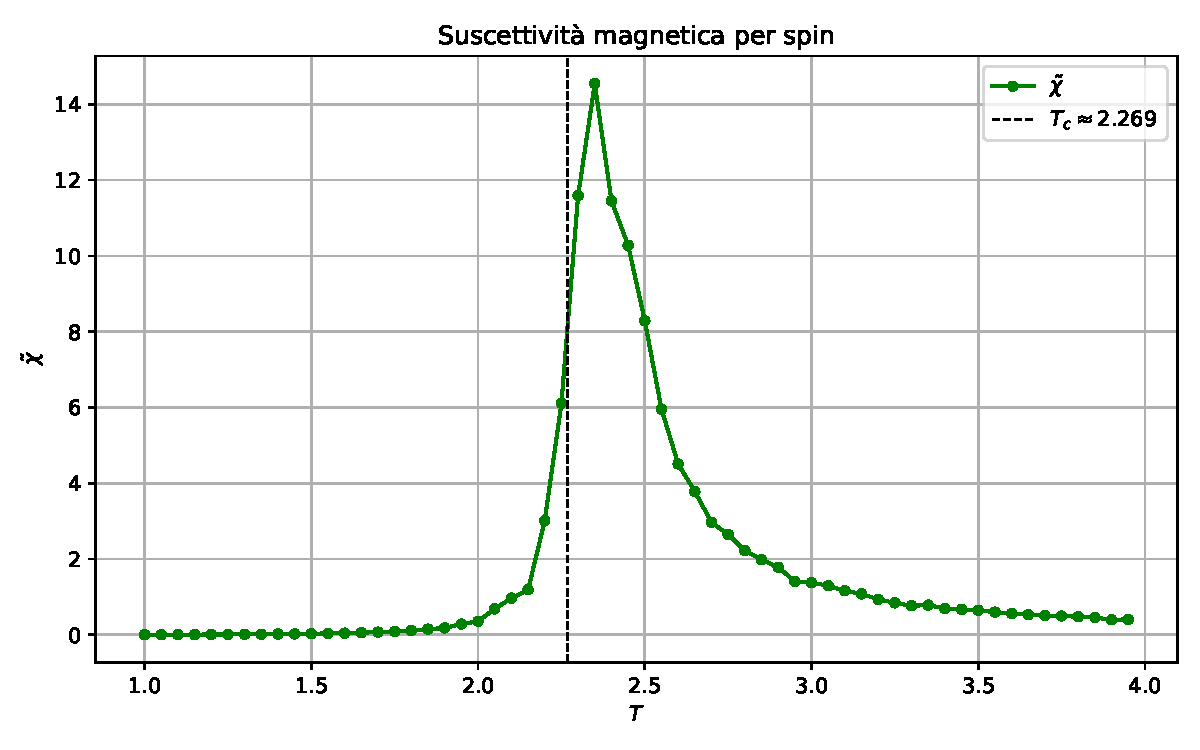
\includegraphics[width=\textwidth]{punto2_chi.pdf}
    \caption{Suscettività magnetica per spin in funzione della temperatura (in unità interne $J=k_B=1$) mediata su $N_{\text{seed}} = 10$ simulazioni indipendenti.}
    \label{fig:chi}
\end{figure}
\FloatBarrier

\subsection{Calore specifico}
In \cref{fig:c} è riportato l'andamento del calore specifico in funzione della temperatura calcolato sia tramite fluttuazioni dell'energia sia tramite derivata numerica simmetrica rispetto alla temperatura.

\begin{figure}[H]
    \centering
    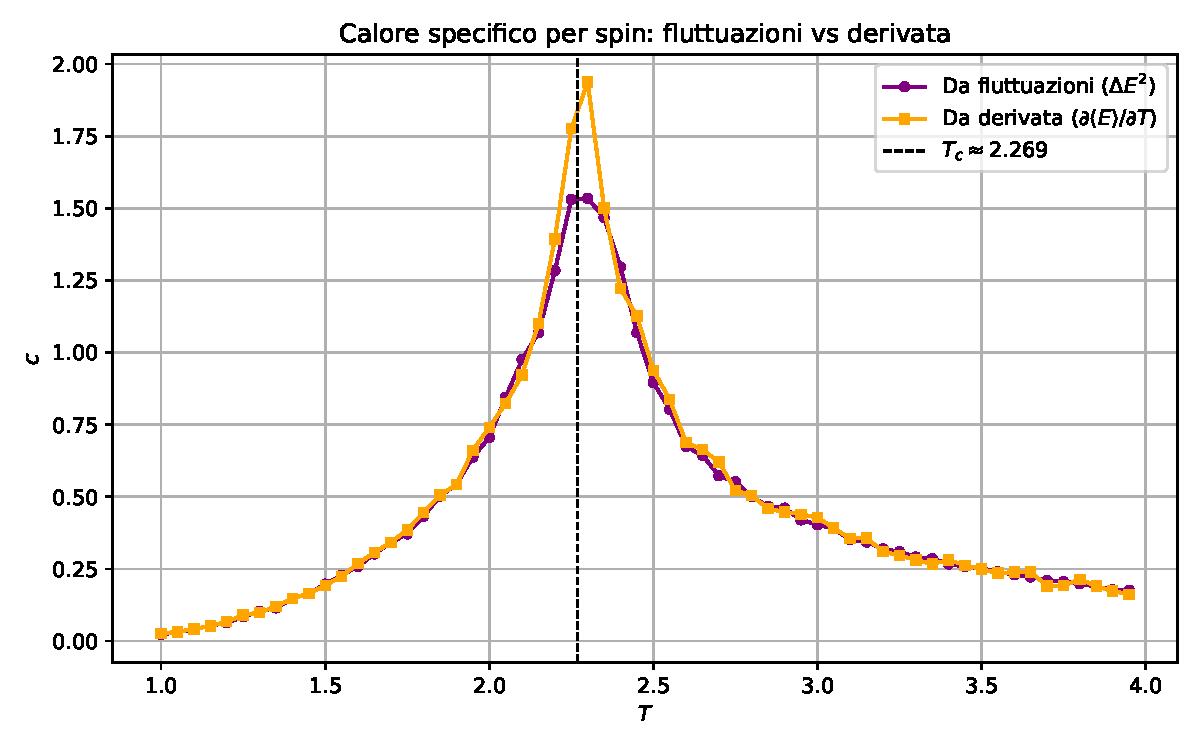
\includegraphics[width=\textwidth]{punto3_c.pdf}
    \caption{Calore specifico calcolato da fluttuazioni dell'energia (viola) e tramite derivata numerica rispetto alla temperatura (giallo) in funzione della temperatura (in unità interne $J=k_B=1$), mediato su $N_{\text{seed}} = 10$ simulazioni indipendenti.}
    \label{fig:c}
\end{figure}
\FloatBarrier

\subsection{Energia e magnetizzazione (sweep completo)}
Ora ridefiniamo lo step Monte Carlo come un intero sweep sequenziale su tutto il reticolo, per un totale di $N_{\text{tot}}=1000$ sweep, scartando i primi $N_{\text{therm}} = 200$ step. Gli andamenti di energia media per spin e magnetizzazione assoluta media per spin sono riportati in \cref{fig:sweep}.

\begin{figure}[H]
    \centering
    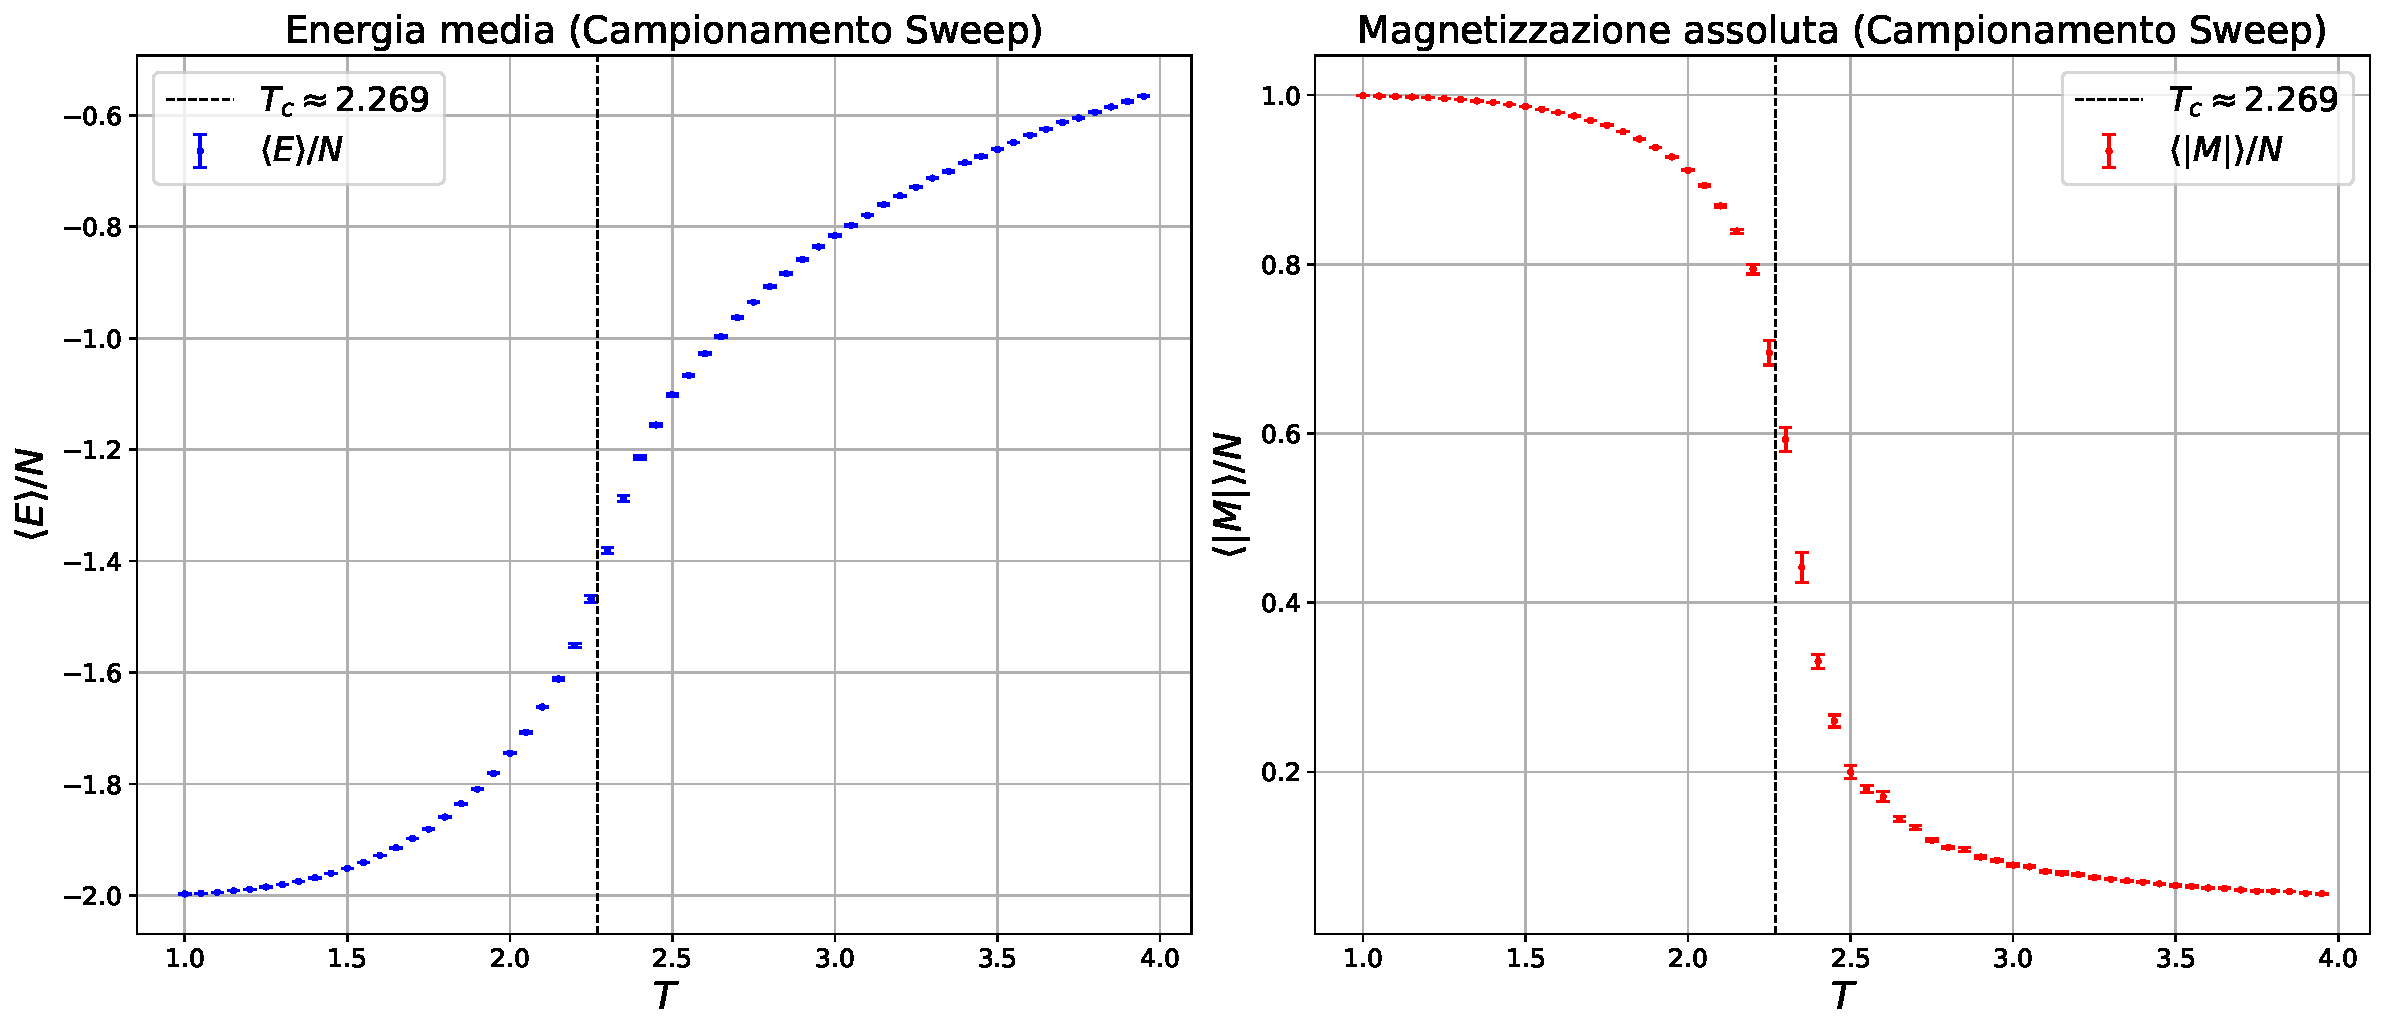
\includegraphics[width=\textwidth]{punto4_sweep.pdf}
    \caption{Energia media per spin (sinistra) e magnetizzazione assoluta media per spin (destra) in funzione della temperatura in unità interne $J=k_B=1$, nel caso in cui uno step Monte Carlo corrisponda ad un intero sweep di tentativi di spin-flip sul reticolo, mediati su $N_{\text{seed}} = 10$ simulazioni indipendenti.}
    \label{fig:sweep}
\end{figure}
\FloatBarrier

\subsection{Autocorrelazione dell'energia}
La funzione di autocorrelazione temporale per l'energia è definita come:
\begin{equation}
    \begin{aligned}
        C_c(\tau) & = \frac{\ev{\delta E(t) \delta E(t + \tau)}}{\ev{(\delta E(t))^2}}                          \\
                  & = \frac{\ev{(E(t) - \ev{E(t)})(E(t + \tau) - \ev{E(t + \tau)})}}{\ev{(E(t) - \ev{E(t)})^2}} \\
        \label{eq:corr}
    \end{aligned}
\end{equation}
Nell'ipotesi stazionaria in cui $\ev{E(t)} = \ev{E(t')}= \bar{E}$ (valida perché vengono scartati i primi $N_{\text{therm}}$ step), dove
\begin{equation}
    \bar{E} = \frac{1}{N_{\text{mis}}} \sum_{t = 0}^{N_{\text{mis}}-1} E(t)
\end{equation}
si ha che \cref{eq:corr} diventa
\begin{equation}
    C_c(\tau)= \frac{\frac{1}{N_{\text{mis}} - \tau} \sum_{t = 0}^{N_{\text{mis}} - \tau - 1} \left(E(t) - \bar{E}\right)\left(E(t + \tau) - \bar{E}\right)}{\frac{1}{N_{\text{mis}}} \sum_{t = 0}^{N_{\text{mis}} - 1} \left(E(t) - \bar{E}\right)^2}
\end{equation}
Infine, si sono mediati i valori della correlazione su $N_{\text{seed}}=10$
\begin{equation}
    C_c(\tau) = \frac{1}{N_{\text{seed}}} \sum_{s = 1}^{N_{\text{seed}}} C_c^{(s)}
\end{equation}

In \cref{fig:autocorrelazione} sono confrontati i due andamenti della funzione di correlazione calcolati con le due diverse definizioni di step Monte Carlo a $T=2$.

\begin{figure}[H]
    \centering
    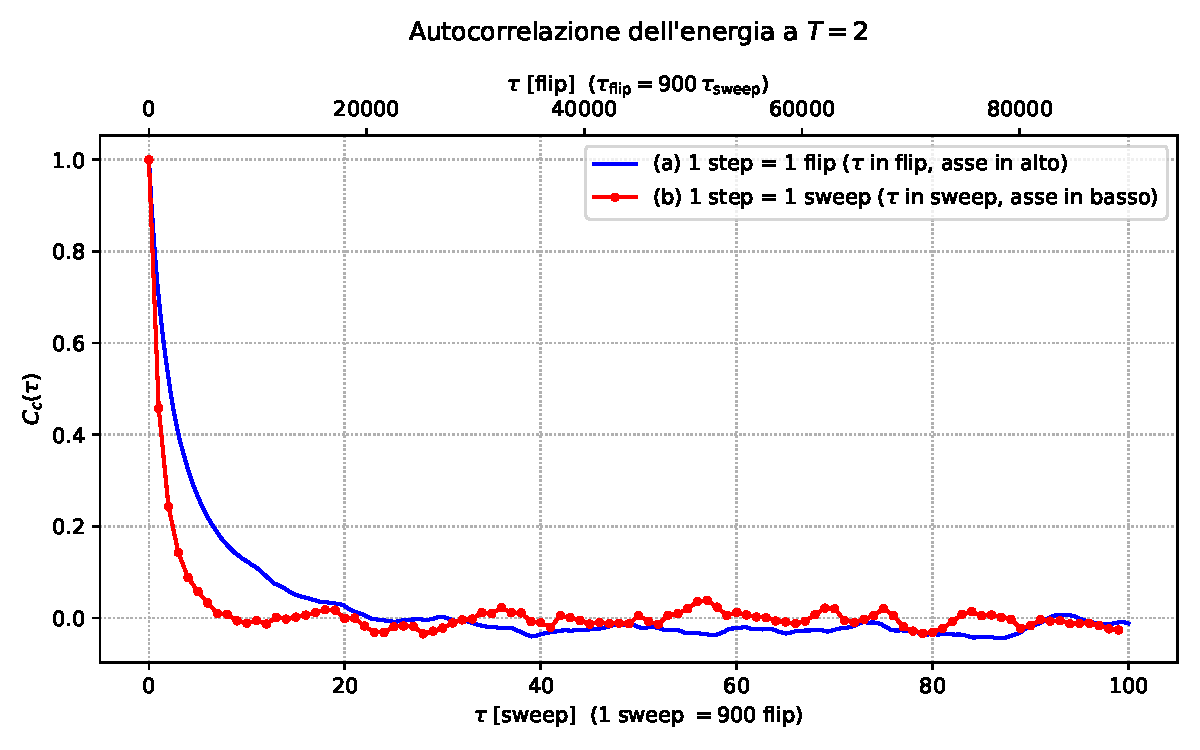
\includegraphics[width=\textwidth]{punto5_autocorrelazione.pdf}
    \caption{Funzione di autocorrelazione normalizzata dell'energia $C_c(\tau)$ a temperatura $T = 2$ (in unità interne $J = k_B = 1$), mediata su $N_{\text{seed}} = 10$ simulazioni indipendenti. Si confrontano la dinamica a singolo tentativo di spin-flip (blu) e quella a sweep completo dell'intero reticolo (rosso).}

    \label{fig:autocorrelazione}
\end{figure}
\FloatBarrier

\section*{Codice}
Il codice sorgente utilizzato per eseguire le simulazioni Monte Carlo e produrre i grafici riportati in questa relazione è disponibile su GitHub al seguente indirizzo:
\begin{center}
    \url{https://github.com/giacomo-cicala/Ising-2D}
\end{center}


\end{document}
